\section{Appendix}

\begin{table}[!htbp]
\caption{Per-class accuracy (\%) on the clean dataset. Columns compare the homogeneous ensemble with its constituent backbones (ResNet-18, ResNet-34, and ResNet-50). The overall row reports aggregate accuracy across classes.}
\label{tab:homo_clean}

\centering
\begin{tabularx}{\linewidth}{lYYYY}
\toprule
Class & {Ensemble} & {ResNet-18} & {ResNet-34} & {ResNet-50} \\
\midrule
binder             & \textbf{98.0} & 96.0 & 86.0 & \textbf{98.0} \\
coffee\_mug        & 78.0 & 78.0 & 76.0 & \textbf{82.0} \\
computer\_keyboard & \textbf{82.0} & \textbf{82.0} & 78.0 & 76.0 \\
mouse              & 78.0 & 66.0 & \textbf{82.0} & 78.0 \\
notebook           & 78.0 & \textbf{86.0} & 80.0 & 82.0 \\
remote\_control    & 94.0 & 90.0 & 92.0 & \textbf{96.0} \\
soup\_bowl         & \textbf{100.0} & 98.0 & 96.0 & 98.0 \\
teapot             & 98.0 & \textbf{100.0} & 96.0 & 98.0 \\
toilet\_tissue     & 90.0 & \textbf{92.0} & 86.0 & 88.0 \\
wooden\_spoon      & 96.0 & 94.0 & 88.0 & \textbf{98.0} \\
\midrule
Overall            & 89.2 & 88.2 & 86.0 & \textbf{89.4} \\
\bottomrule
\end{tabularx}

\end{table}

\begin{table}[!htbp]
\caption{Per-class accuracy (\%) on the clean dataset. Columns compare the heterogeneous ensemble with its constituent backbones (DenseNet-121, EfficientNet-B0, ResNet-34, and ViT-B/16). The overall row reports aggregate accuracy across classes.}
\label{tab:hetero_clean}

\centering
\begin{tabularx}{\linewidth}{lYYYYY}
\toprule
Class & {Ensemble} & {DenseNet121} & {EfficientNet} & {ResNet-34} & {ViT-B/16} \\
\midrule
binder             & \textbf{100.0} & 94.0 & 96.0 & 94.0 & \textbf{100.0} \\
coffee\_mug        & 82.0 & 78.0 & 76.0 & 82.0 & \textbf{84.0} \\
computer\_keyboard & 86.0 & 76.0 & 76.0 & 80.0 & \textbf{88.0} \\
mouse              & 80.0 & 74.0 & 82.0 & 72.0 & \textbf{86.0} \\
notebook           & 84.0 & 82.0 & \textbf{86.0} & 82.0 & 80.0 \\
remote\_control    & \textbf{96.0} & 94.0 & \textbf{96.0} & 88.0 & \textbf{96.0} \\
soup\_bowl         & \textbf{98.0} & \textbf{98.0} & 96.0 & \textbf{98.0} & 94.0 \\
teapot             & \textbf{100.0} & 98.0 & \textbf{100.0} & 96.0 & \textbf{100.0} \\
toilet\_tissue     & \textbf{96.0} & 92.0 & 94.0 & 92.0 & 94.0 \\
wooden\_spoon      & \textbf{96.0} & \textbf{96.0} & 94.0 & 94.0 & 94.0 \\
\midrule
Overall            & \textbf{91.8} & 88.2 & 89.6 & 87.8 & 91.6 \\
\bottomrule
\end{tabularx}

\end{table}

\begin{figure}[!htbp]
  \centering
  \fbox{%
    \rule[-.5cm]{0cm}{0cm}%
    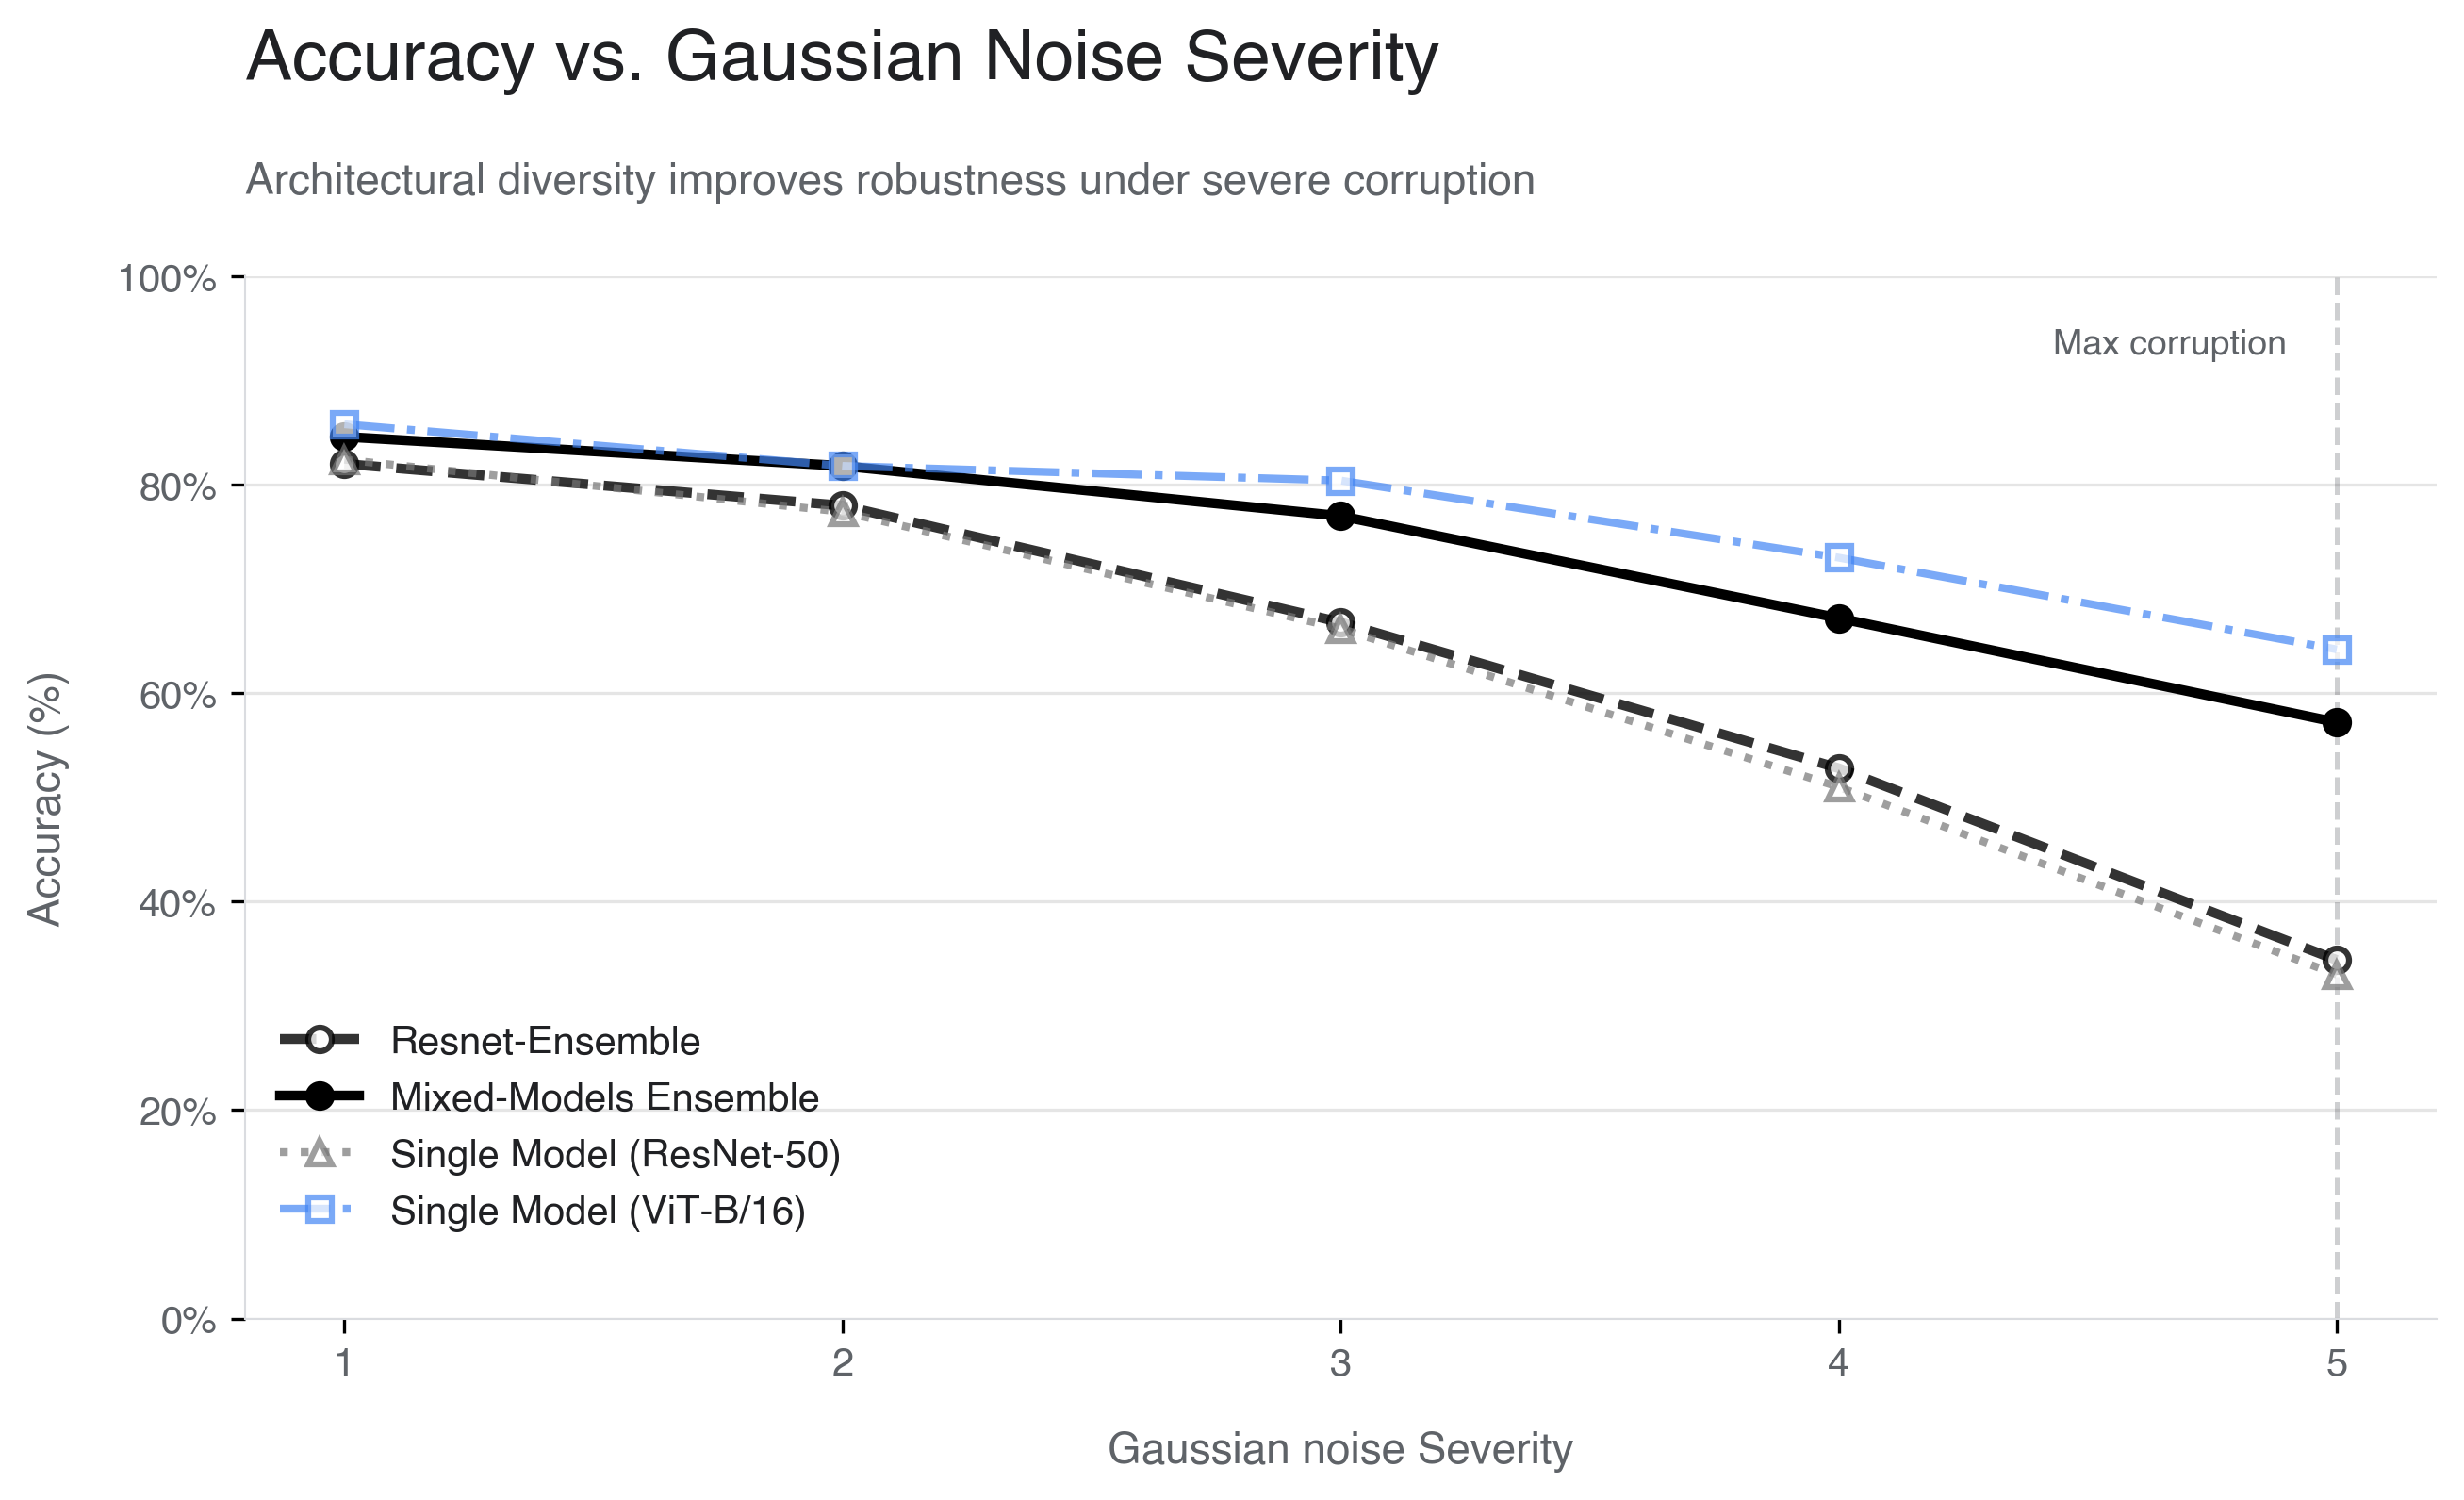
\includegraphics[width=1\linewidth]{xAI-StudentReportTemplate/figures/ensemble_noise_robustness.png}%
    \rule[-.5cm]{0cm}{0cm}%
  }
  \caption{Classification accuracy under Gaussian noise corruption across five severity levels. Results are shown for a homogeneous ResNet ensemble, the heterogeneous mixed-model ensemble, and the strongest single backbones (ResNet-50 and ViT-B/16). Evaluation is performed on the synthetic corruption benchmark.}
  \label{fig:appendix_gaussian}
\end{figure}

\begin{figure}[!htbp]
  \centering
  \fbox{%
    \rule[-.5cm]{0cm}{0cm}%
    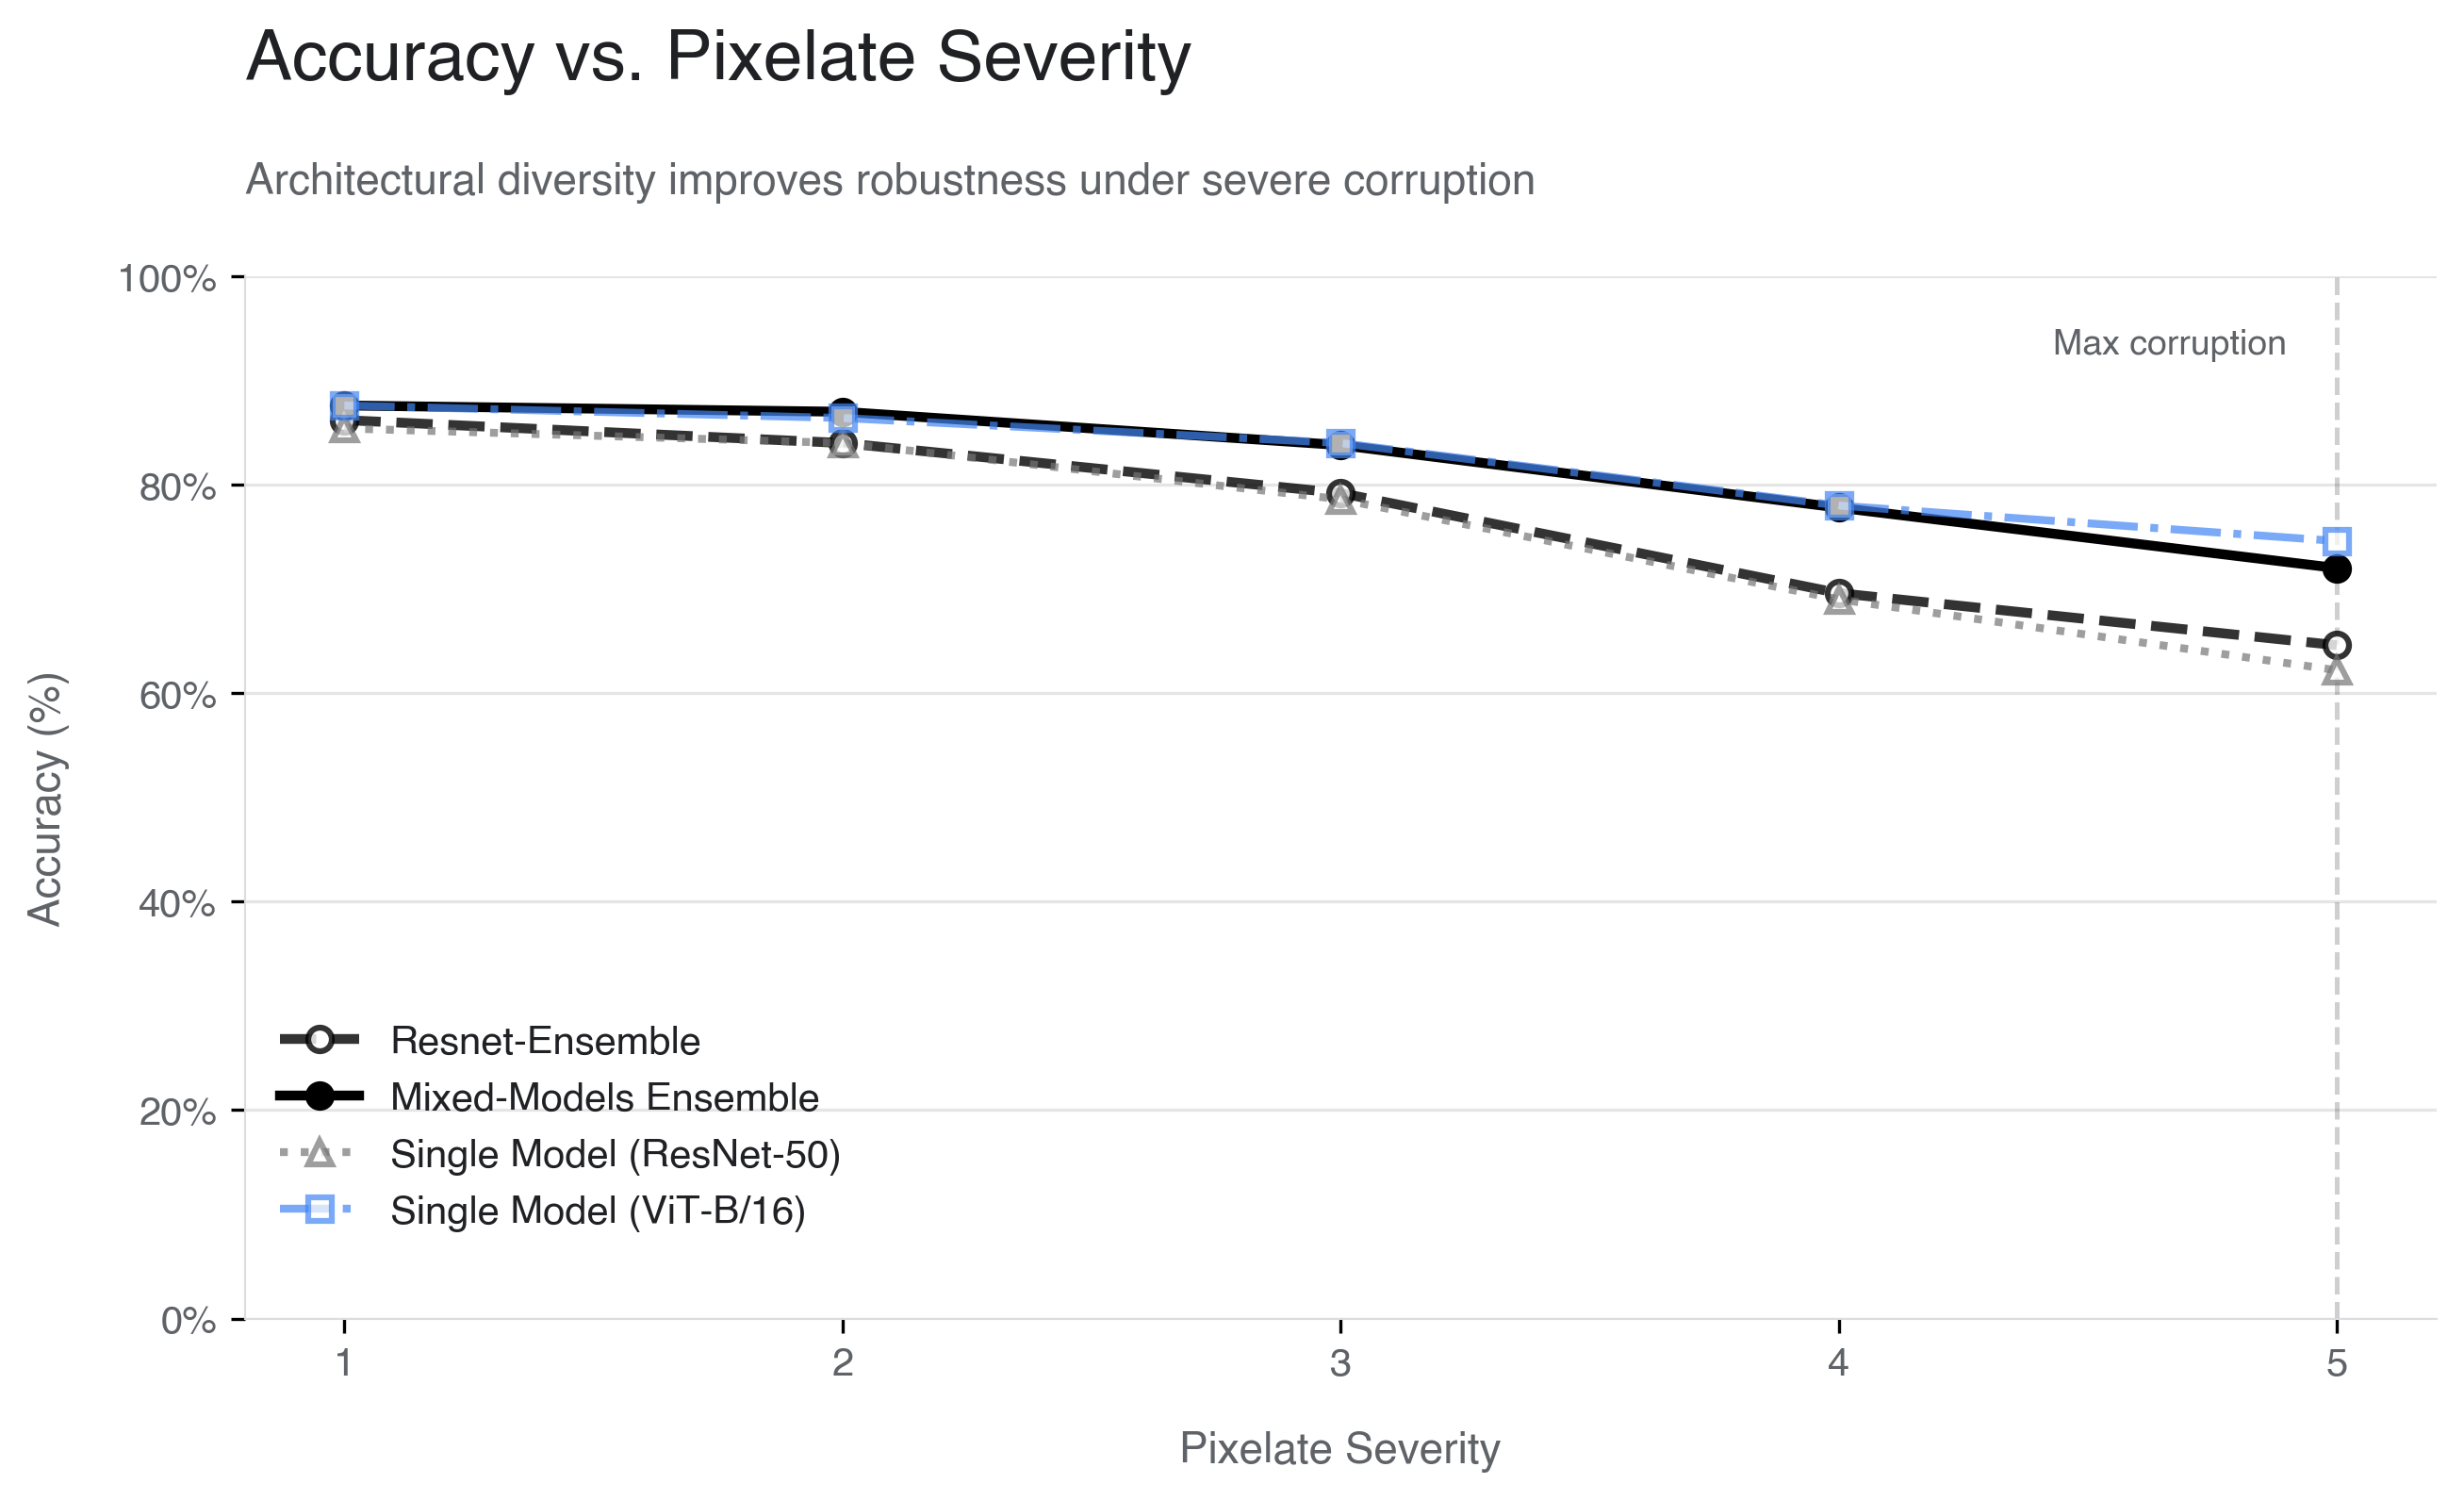
\includegraphics[width=1\linewidth]{xAI-StudentReportTemplate/figures/ensemble_pixelate_robustness.png}%
    \rule[-.5cm]{0cm}{0cm}%
  }
  \caption{Classification accuracy under pixelation corruption across five severity levels. Results are shown for a homogeneous ResNet ensemble, the heterogeneous mixed-model ensemble, and the strongest single backbones (ResNet-50 and ViT-B/16). All evaluations are conducted on the synthetic corruption benchmark.}
  \label{fig:appendix_pixelate}
\end{figure}

\begin{table}[!htbp]
\caption{Per-class accuracy (\%) on the phone-captured out-of-distribution dataset. Columns compare the homogeneous ensemble with its constituent backbones (ResNet-18, ResNet-34, and ResNet-50). The overall row reports aggregate accuracy across classes.}
\label{tab:homo_phone}

\centering
\begin{tabularx}{\linewidth}{lYYYY}
\toprule
Class & {Ensemble} & {ResNet-18} & {ResNet-34} & {ResNet-50} \\
\midrule
binder             & 55.3 & 51.5 & 45.6 & \textbf{58.4} \\
coffee\_mug        & 48.5 & 42.7 & 39.7 & \textbf{54.9} \\
computer\_keyboard & 42.6 & 39.6 & 36.8 & \textbf{44.7} \\
mouse              & 52.9 & 46.7 & \textbf{56.3} & 48.7 \\
notebook           & \textbf{66.0} & 62.5 & 60.0 & 64.9 \\
remote\_control    & 62.7 & 52.9 & 58.8 & \textbf{64.0} \\
soup\_bowl         & 34.3 & 30.4 & 30.8 & \textbf{35.3} \\
teapot             & 37.1 & 32.7 & \textbf{40.0} & 35.8 \\
toilet\_tissue     & 77.9 & \textbf{78.8} & 70.3 & 75.1 \\
wooden\_spoon      & 81.2 & 74.1 & 78.2 & \textbf{81.4} \\
\midrule
Overall            & 55.8 & 51.1 & 51.6 & \textbf{56.3} \\
\bottomrule
\end{tabularx}

\end{table}

\begin{table}[!htbp]
\caption{Per-class accuracy (\%) on the phone-captured out-of-distribution dataset. Columns compare the heterogeneous ensemble with its constituent backbones (DenseNet-121, EfficientNet-B0, ResNet-34, and ViT-B/16). The overall row reports aggregate accuracy across classes.}
\label{tab:hetero_phone}

\centering
\begin{tabularx}{\linewidth}{lYYYYY}
\toprule
Class & {Ensemble} & {DenseNet121} & {EfficientNet} & {ResNet-34} & {ViT-B/16} \\
\midrule
binder             & 56.9 & 38.2 & 51.7 & 48.5 & \textbf{68.3} \\
coffee\_mug        & 49.1 & 48.5 & 41.2 & 38.6 & \textbf{57.1} \\
computer\_keyboard & 44.3 & 39.3 & 33.0 & 37.7 & \textbf{54.8} \\
mouse              & 49.2 & 46.9 & \textbf{49.4} & 41.9 & 43.5 \\
notebook           & 74.0 & 71.9 & \textbf{74.5} & 62.3 & 67.0 \\
remote\_control    & 57.5 & 54.4 & 55.7 & 44.3 & \textbf{60.5} \\
soup\_bowl         & \textbf{32.5} & 29.7 & 30.6 & 24.8 & 32.0 \\
teapot             & 44.8 & 38.0 & 41.7 & 40.6 & \textbf{49.2} \\
toilet\_tissue     & \textbf{86.4} & 82.5 & 74.0 & 80.6 & 84.3 \\
wooden\_spoon      & \textbf{86.0} & 81.4 & 84.6 & 81.2 & 84.6 \\
\midrule
Overall            & 58.0 & 53.0 & 53.6 & 49.9 & \textbf{60.1} \\
\bottomrule
\end{tabularx}

\end{table}

\begin{figure}[!htbp]
  \centering
  \fbox{%
    \rule[-.5cm]{0cm}{0cm}%
    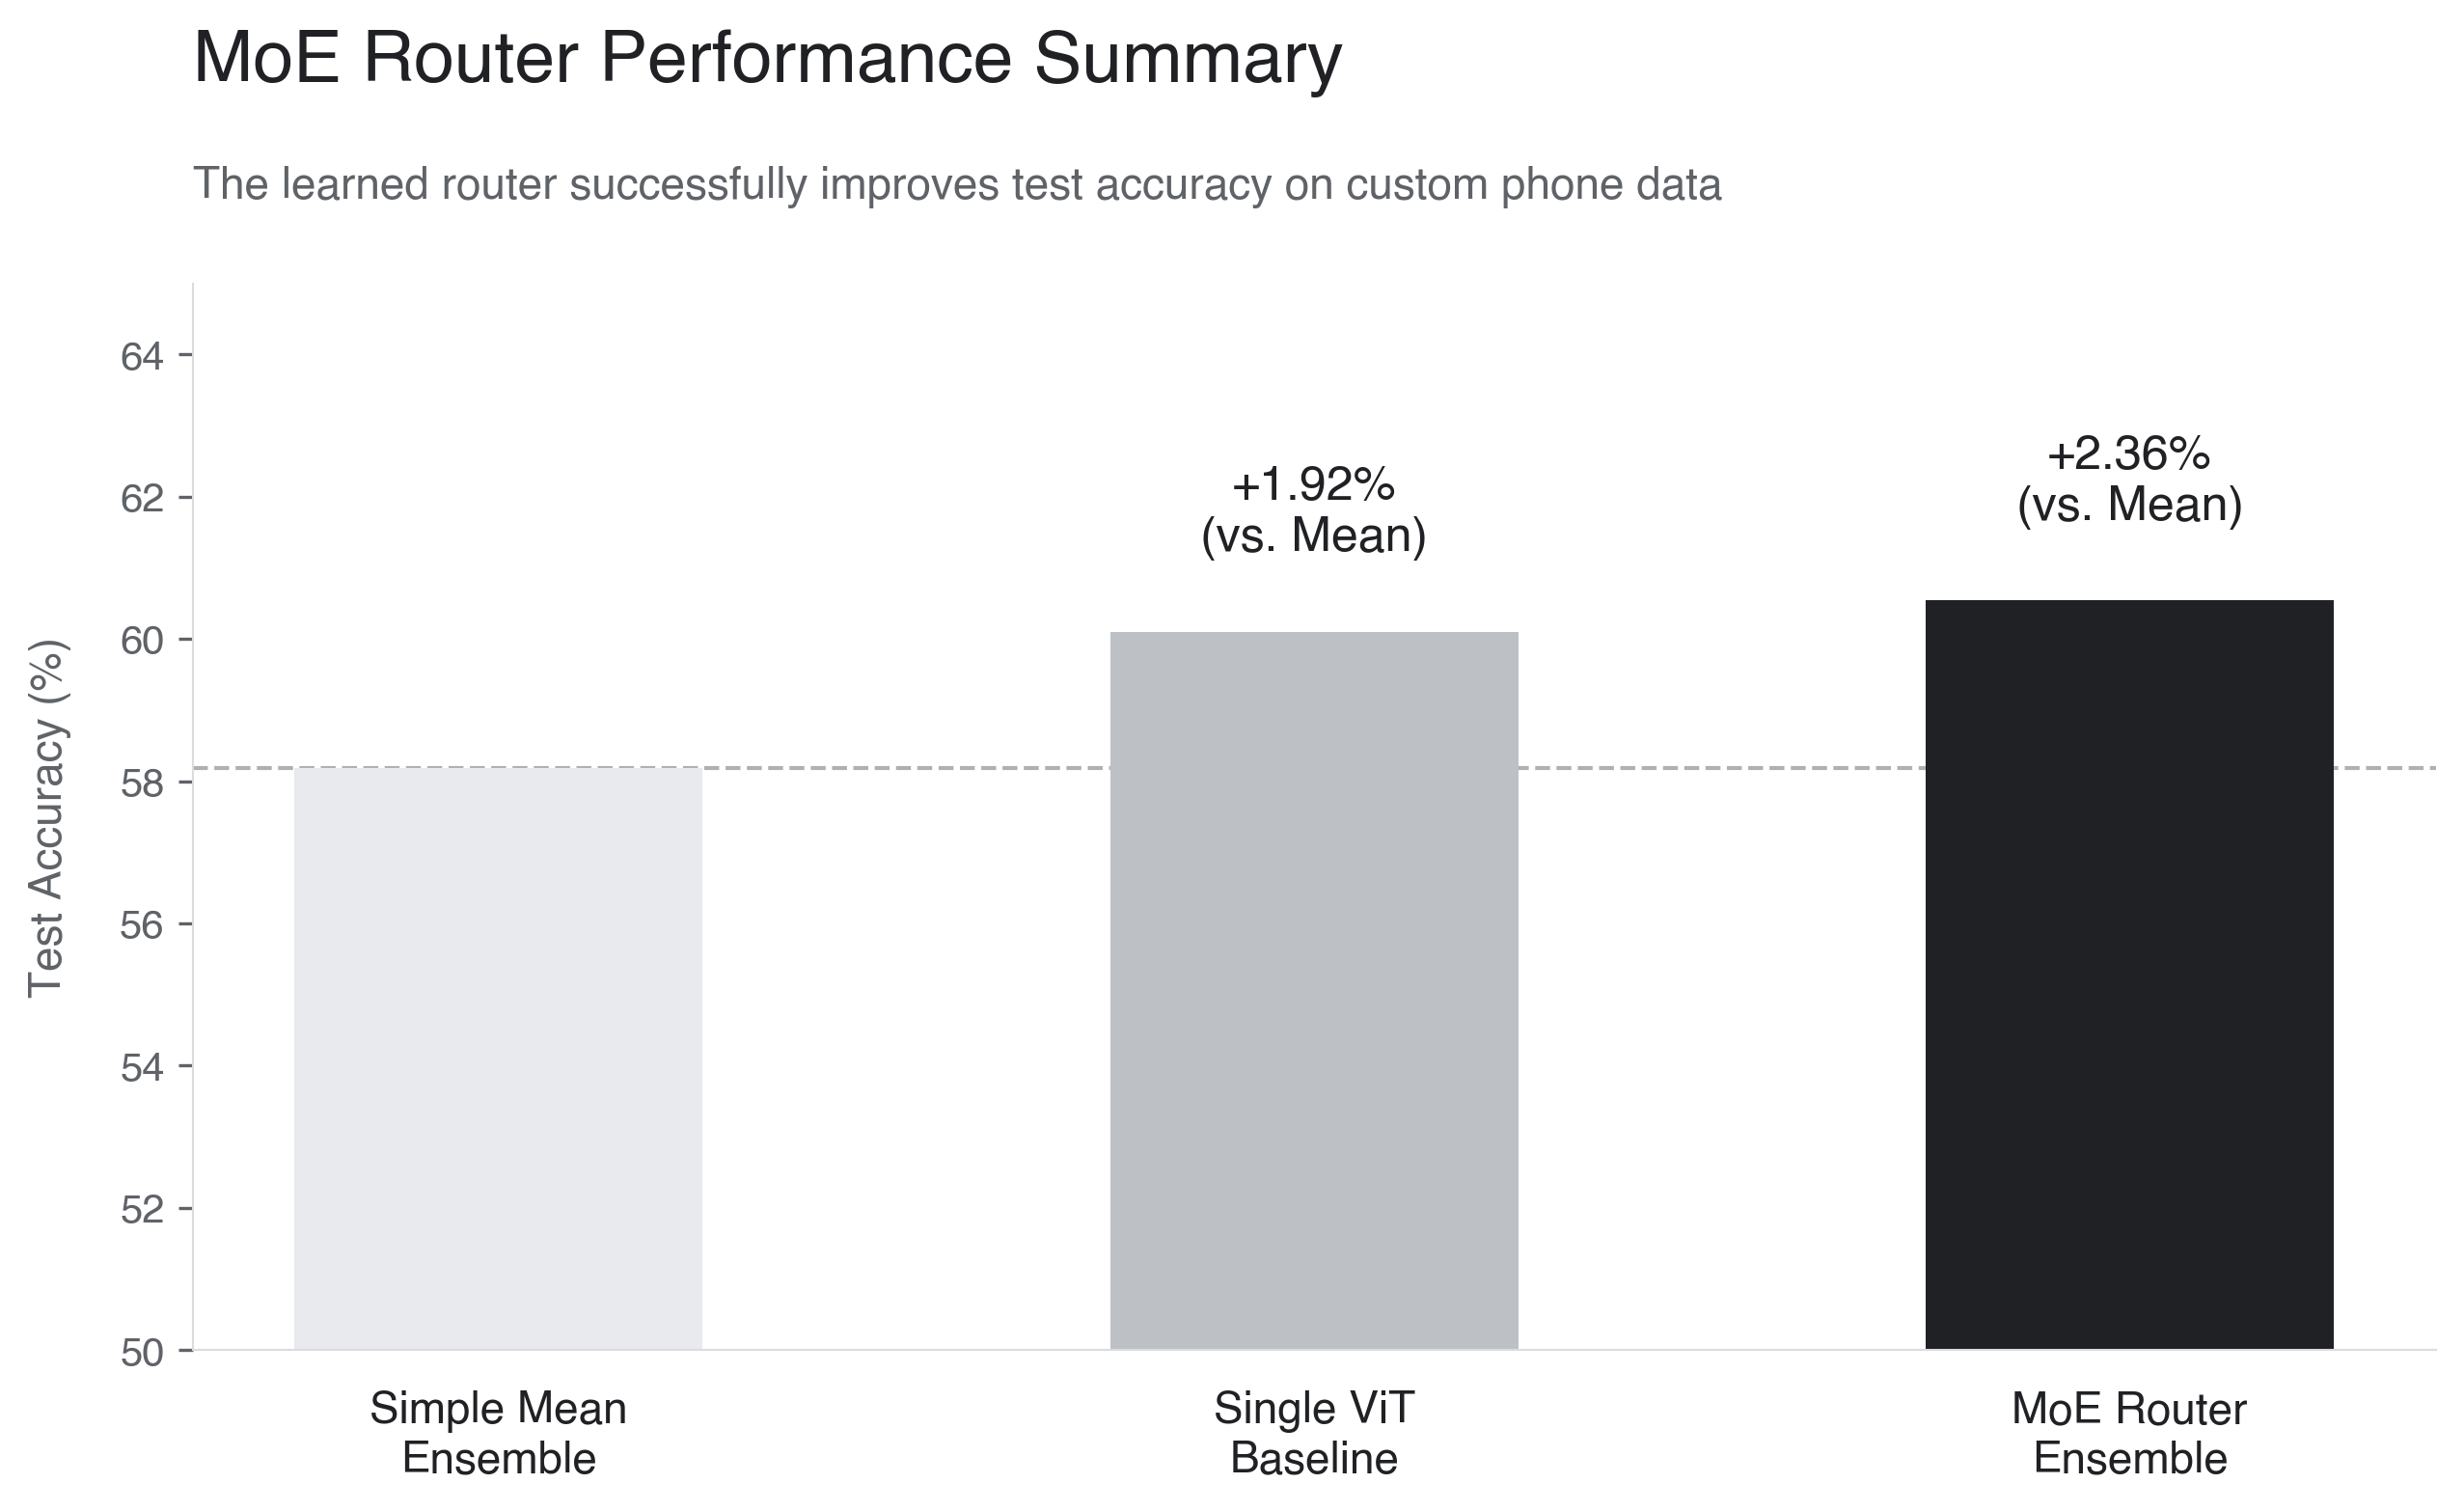
\includegraphics[width=1\linewidth]{xAI-StudentReportTemplate/figures/moe_router_improvement.png}%
    \rule[-.5cm]{0cm}{0cm}%
  }
  \caption{Test accuracy on the phone-captured dataset for uniform averaging (Simple Mean Ensemble), the strongest single backbone (ViT-B/16), and the Mixture-of-Experts (MoE) router. Percentage annotations indicate relative improvement over uniform averaging.}
  \label{fig:moe_improve}
\end{figure}

\begin{figure}[!htbp]
  \centering
  \fbox{%
    \rule[-.5cm]{0cm}{0cm}%
    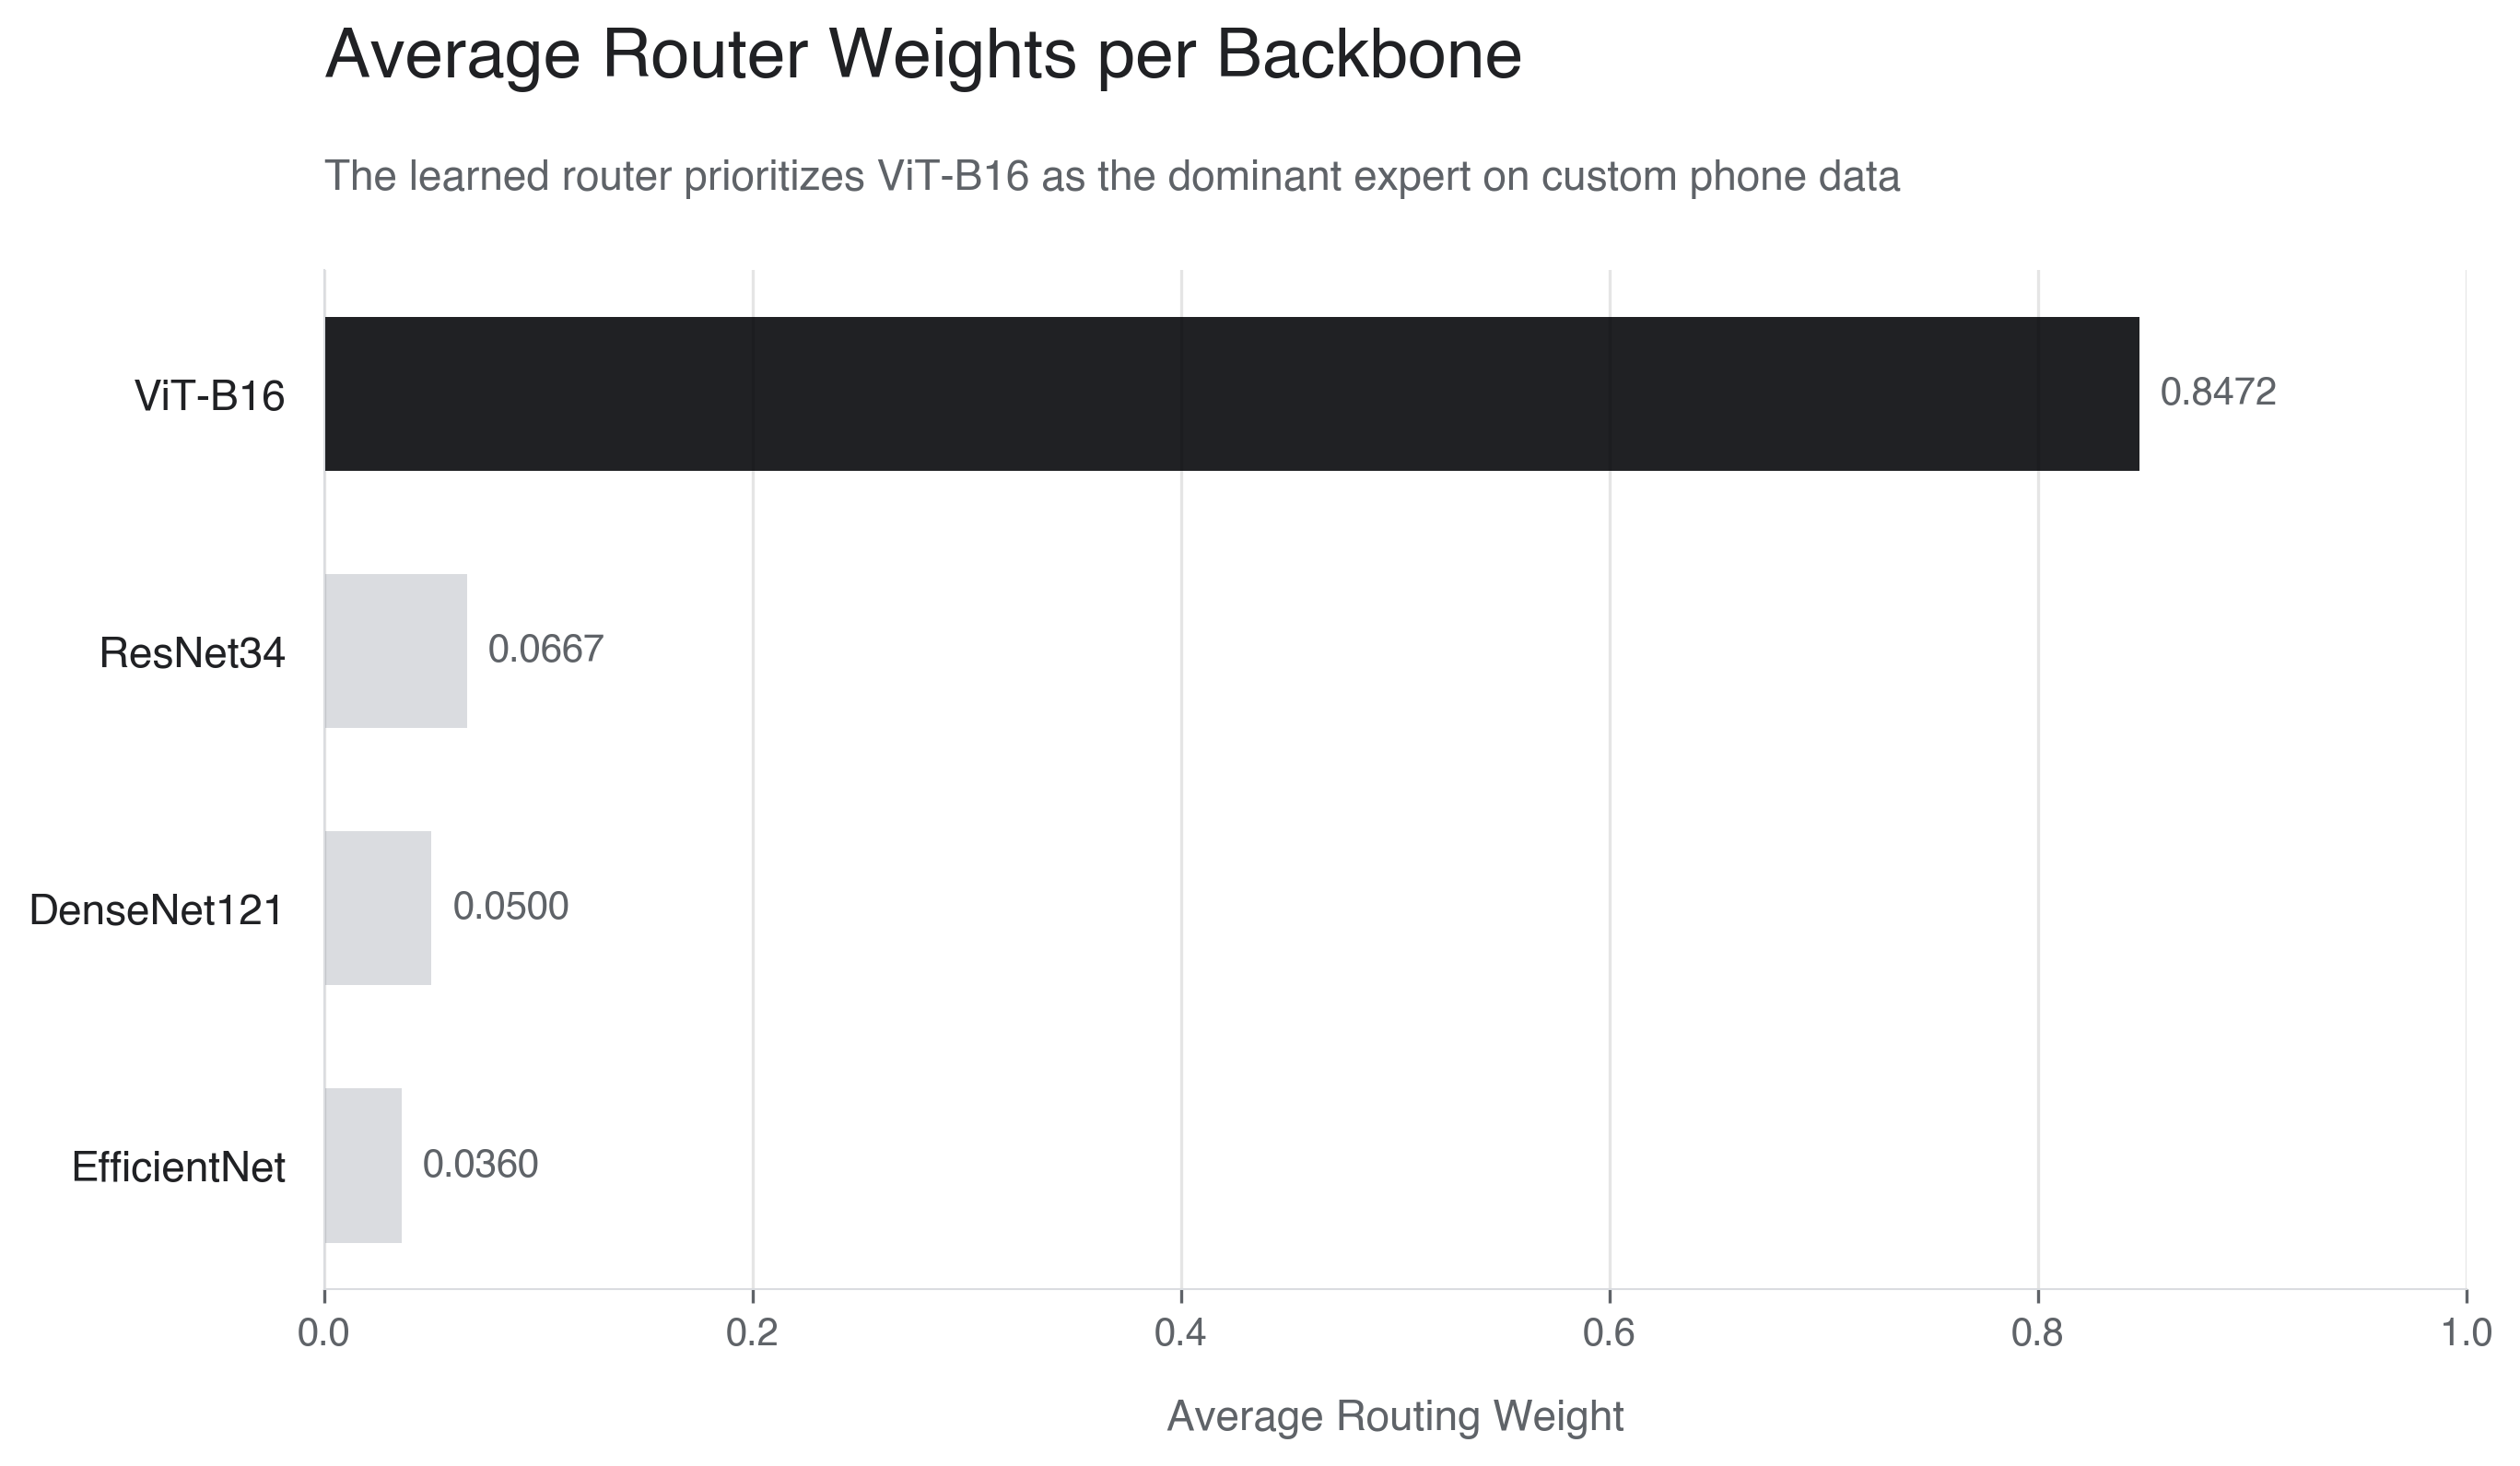
\includegraphics[width=1\linewidth]{xAI-StudentReportTemplate/figures/router_weights_summary.png}%
    \rule[-.5cm]{0cm}{0cm}%
  }
  \caption{Average routing weight assigned to each backbone by the mixture-of-experts router on the phone-captured dataset.
    Weights are averaged across all samples. The router assigns the majority of probability mass to the ViT-B/16 backbone.}
  \label{fig:moe_weights}
\end{figure}

\begin{figure}[!htbp]
  \centering
  \fbox{%
    \rule[-.5cm]{0cm}{0cm}%
    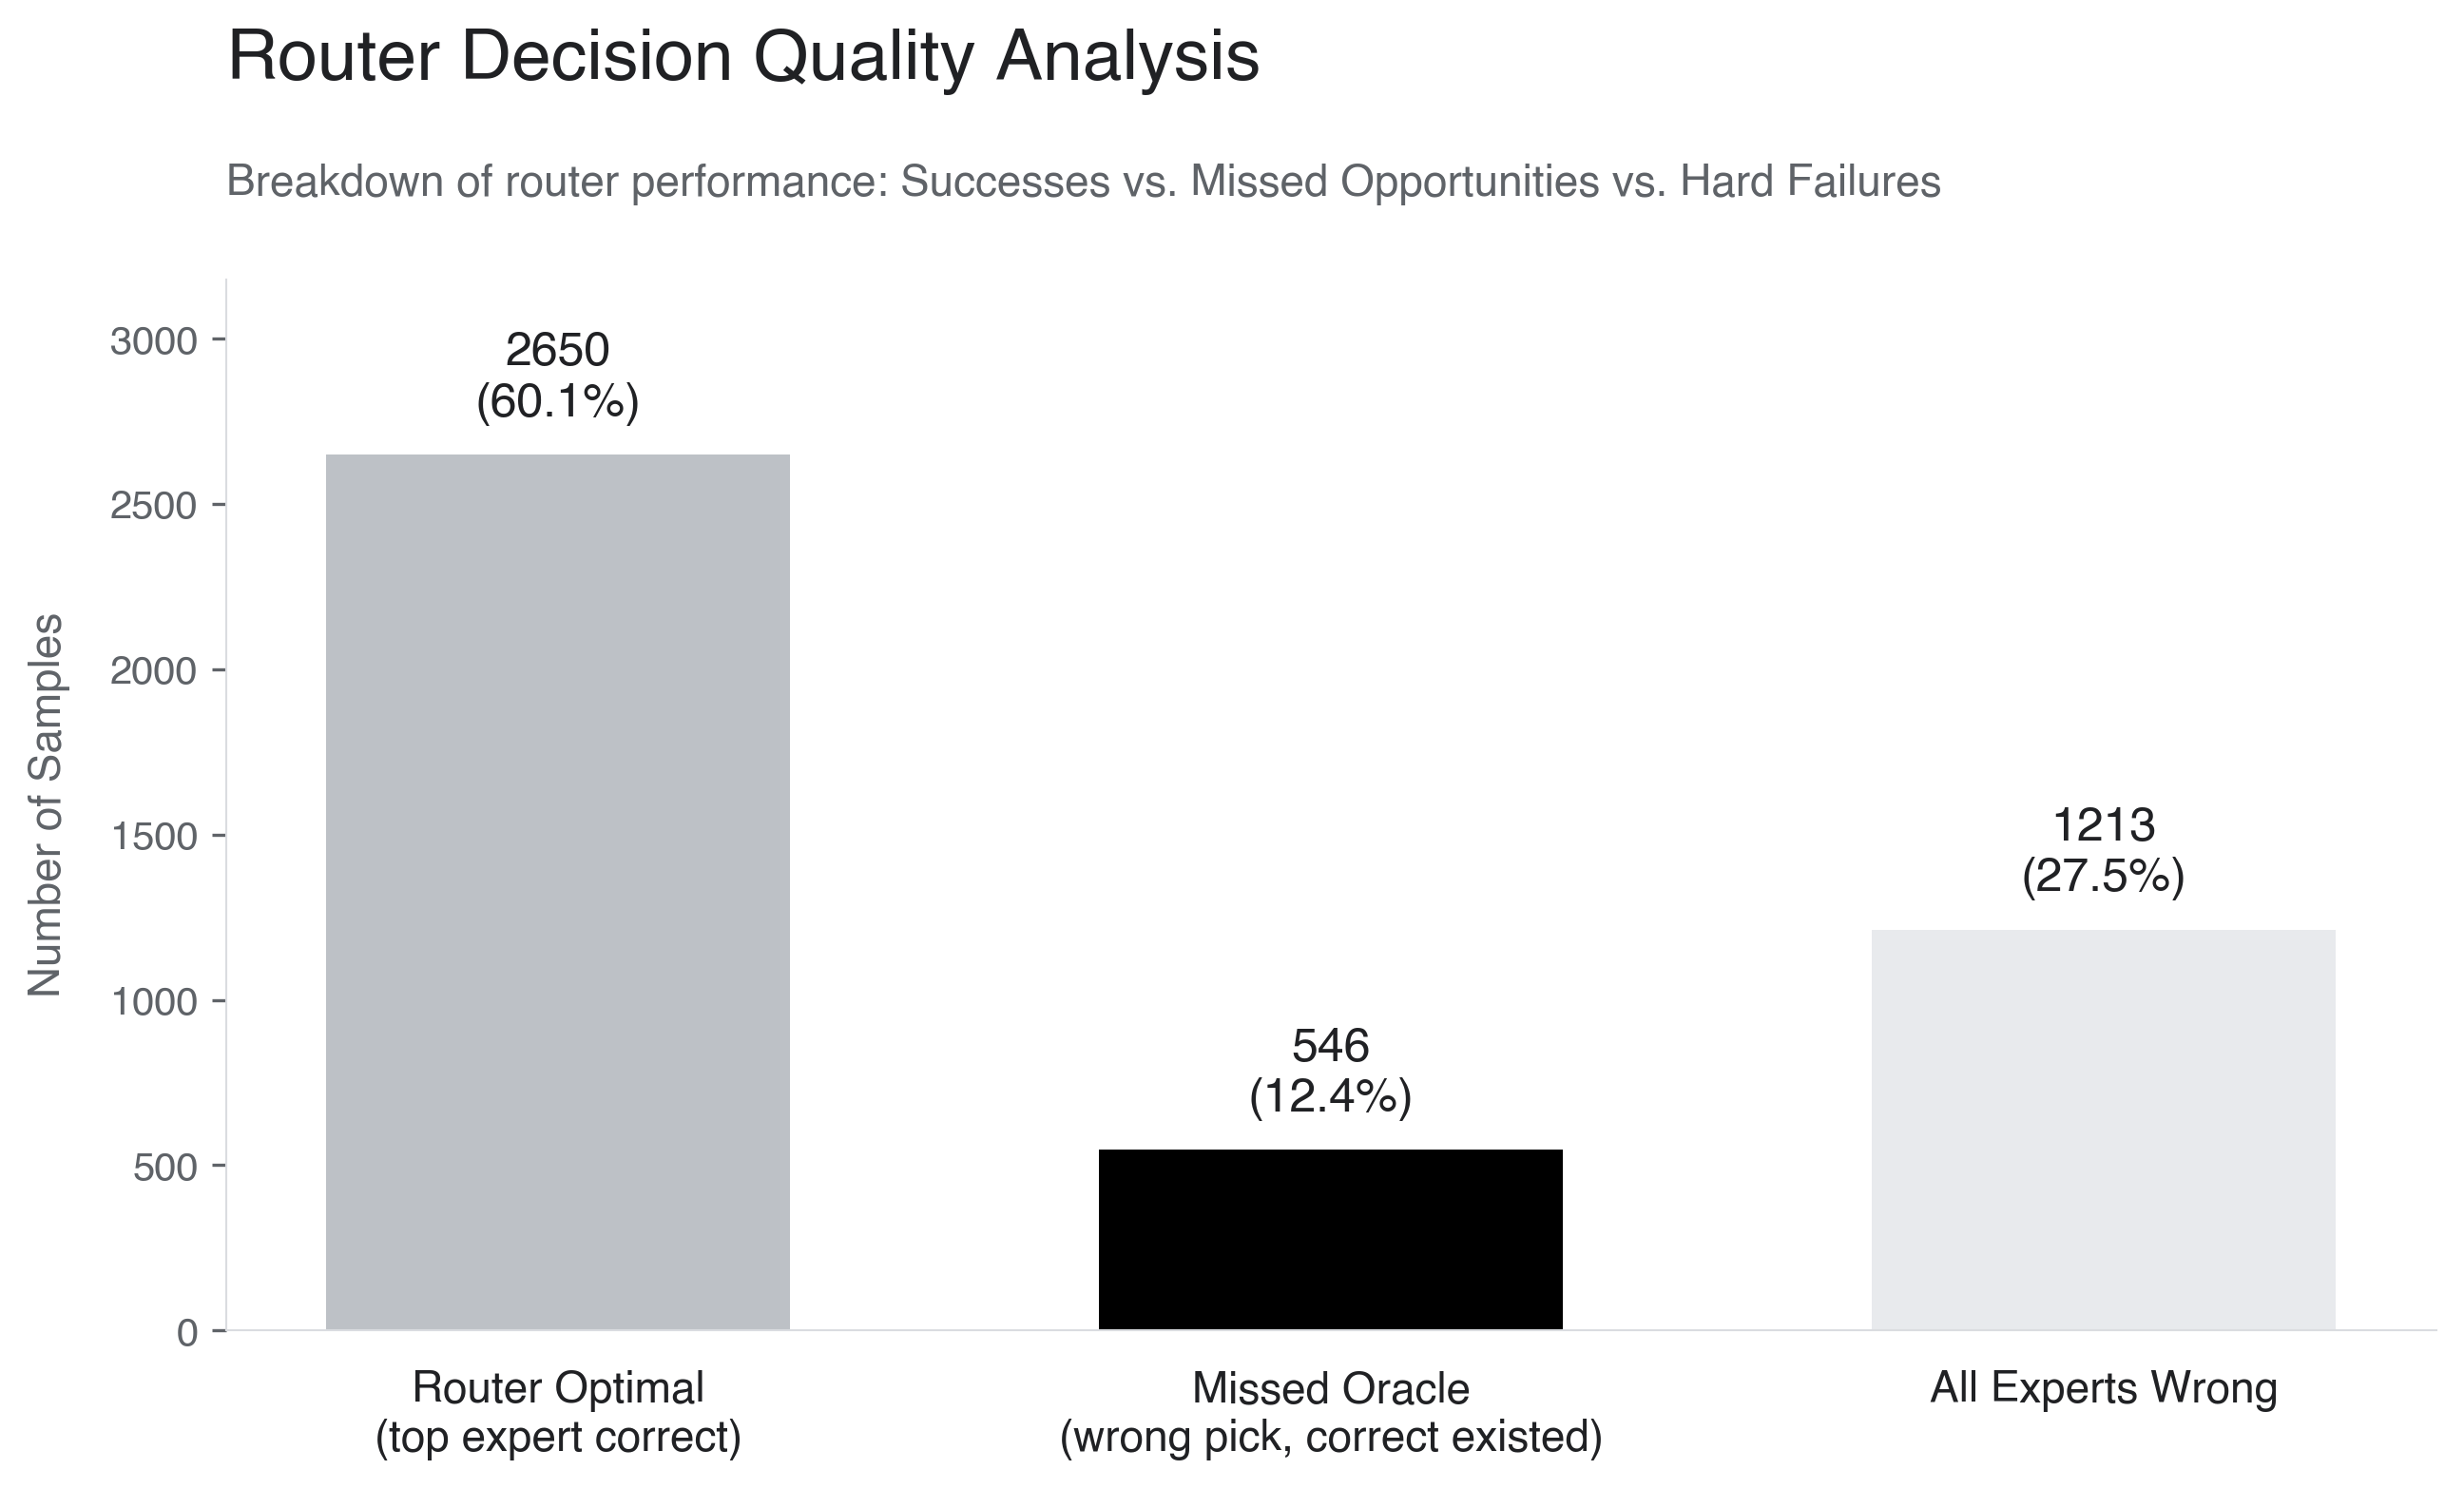
\includegraphics[width=1\linewidth]{xAI-StudentReportTemplate/figures/router_quality_plot.png}%
    \rule[-.5cm]{0cm}{0cm}%
  }
  \caption{Breakdown of routing outcomes on the phone-captured dataset. Samples are categorized as: (i) router selects a correct expert (“Router Optimal”), (ii) router selects an incorrect expert although another expert predicts correctly (“Missed Oracle”), and (iii) all experts predict incorrectly (“All Experts Wrong”). Percentages indicate the proportion of total evaluation samples in each category.}
  \label{fig:moe_missed}
\end{figure}

\begin{figure}[!htbp]
  \centering
  \fbox{%
    \rule[-.5cm]{0cm}{0cm}%
    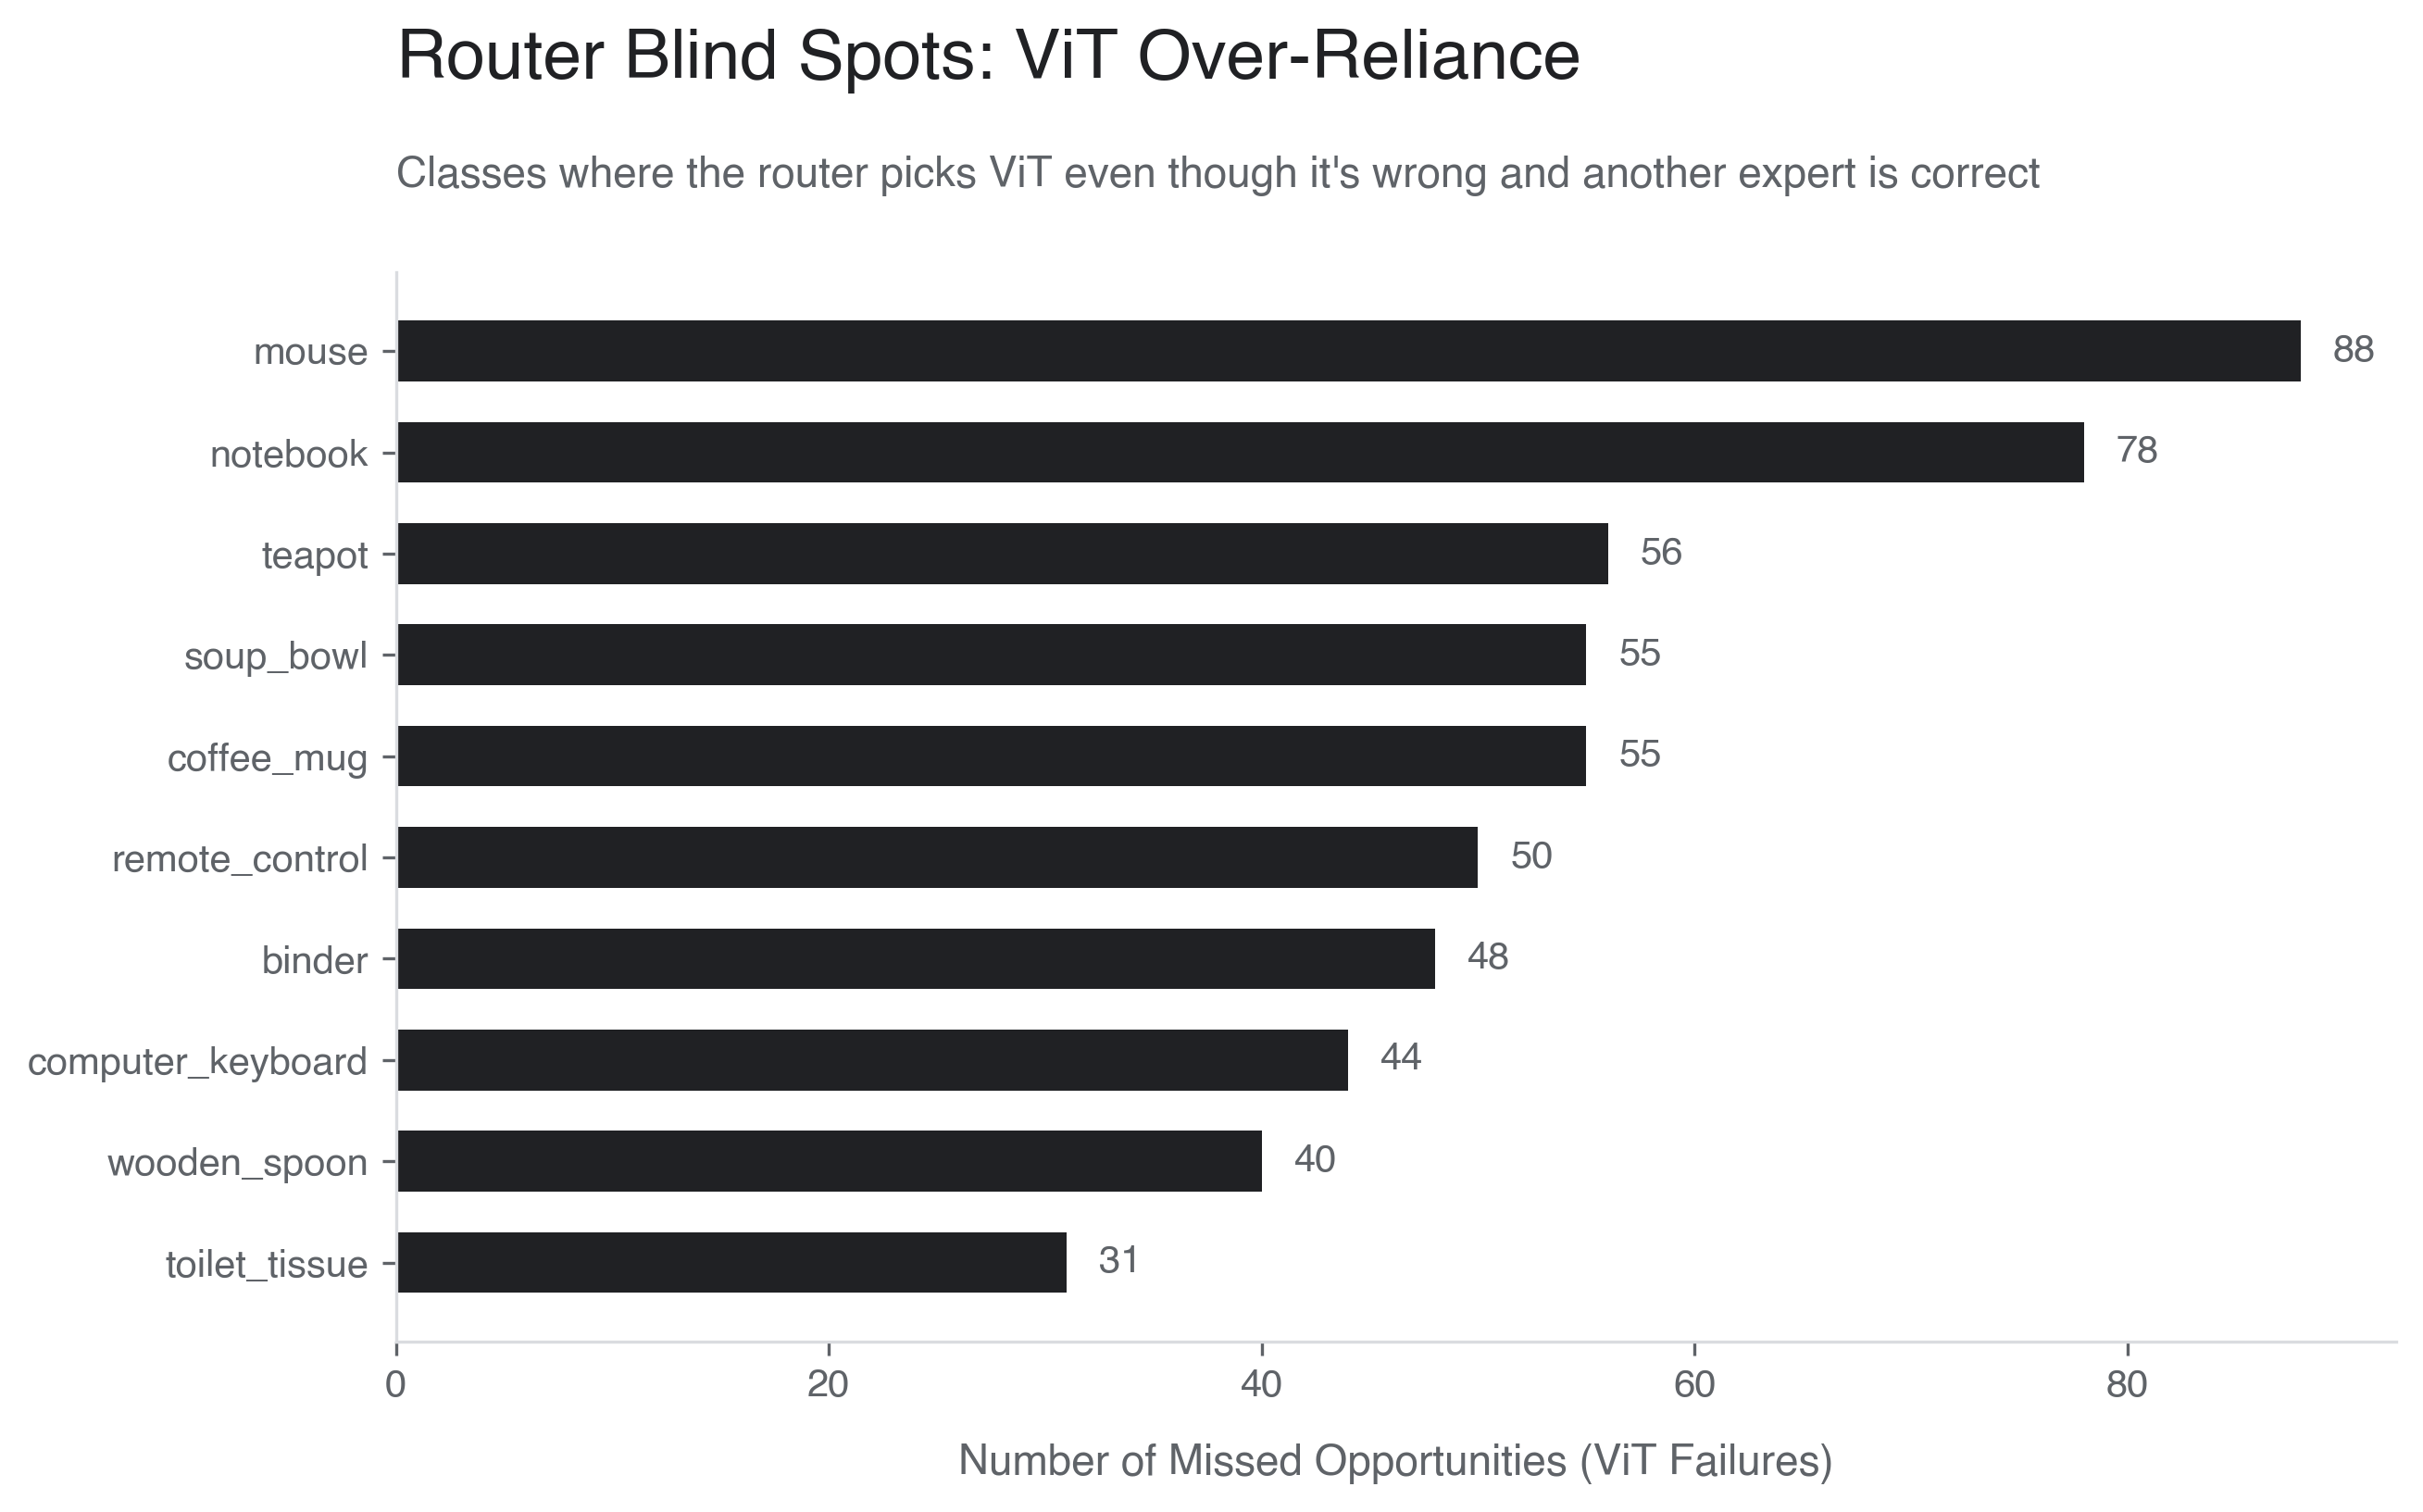
\includegraphics[width=1\linewidth]{xAI-StudentReportTemplate/figures/vit_over_reliance_failure.png}
    \rule[-.5cm]{0cm}{0cm}%
  }
  \caption{Class-wise distribution of missed oracle cases on the phone-captured dataset.
    The bars indicate the number of samples per class where the router selects the ViT backbone despite another expert predicting correctly.}
  \label{fig:vit_fails}
\end{figure}

\begin{figure}[!htbp]
  \centering
  \fbox{%
    \rule[-.5cm]{0cm}{0cm}%
    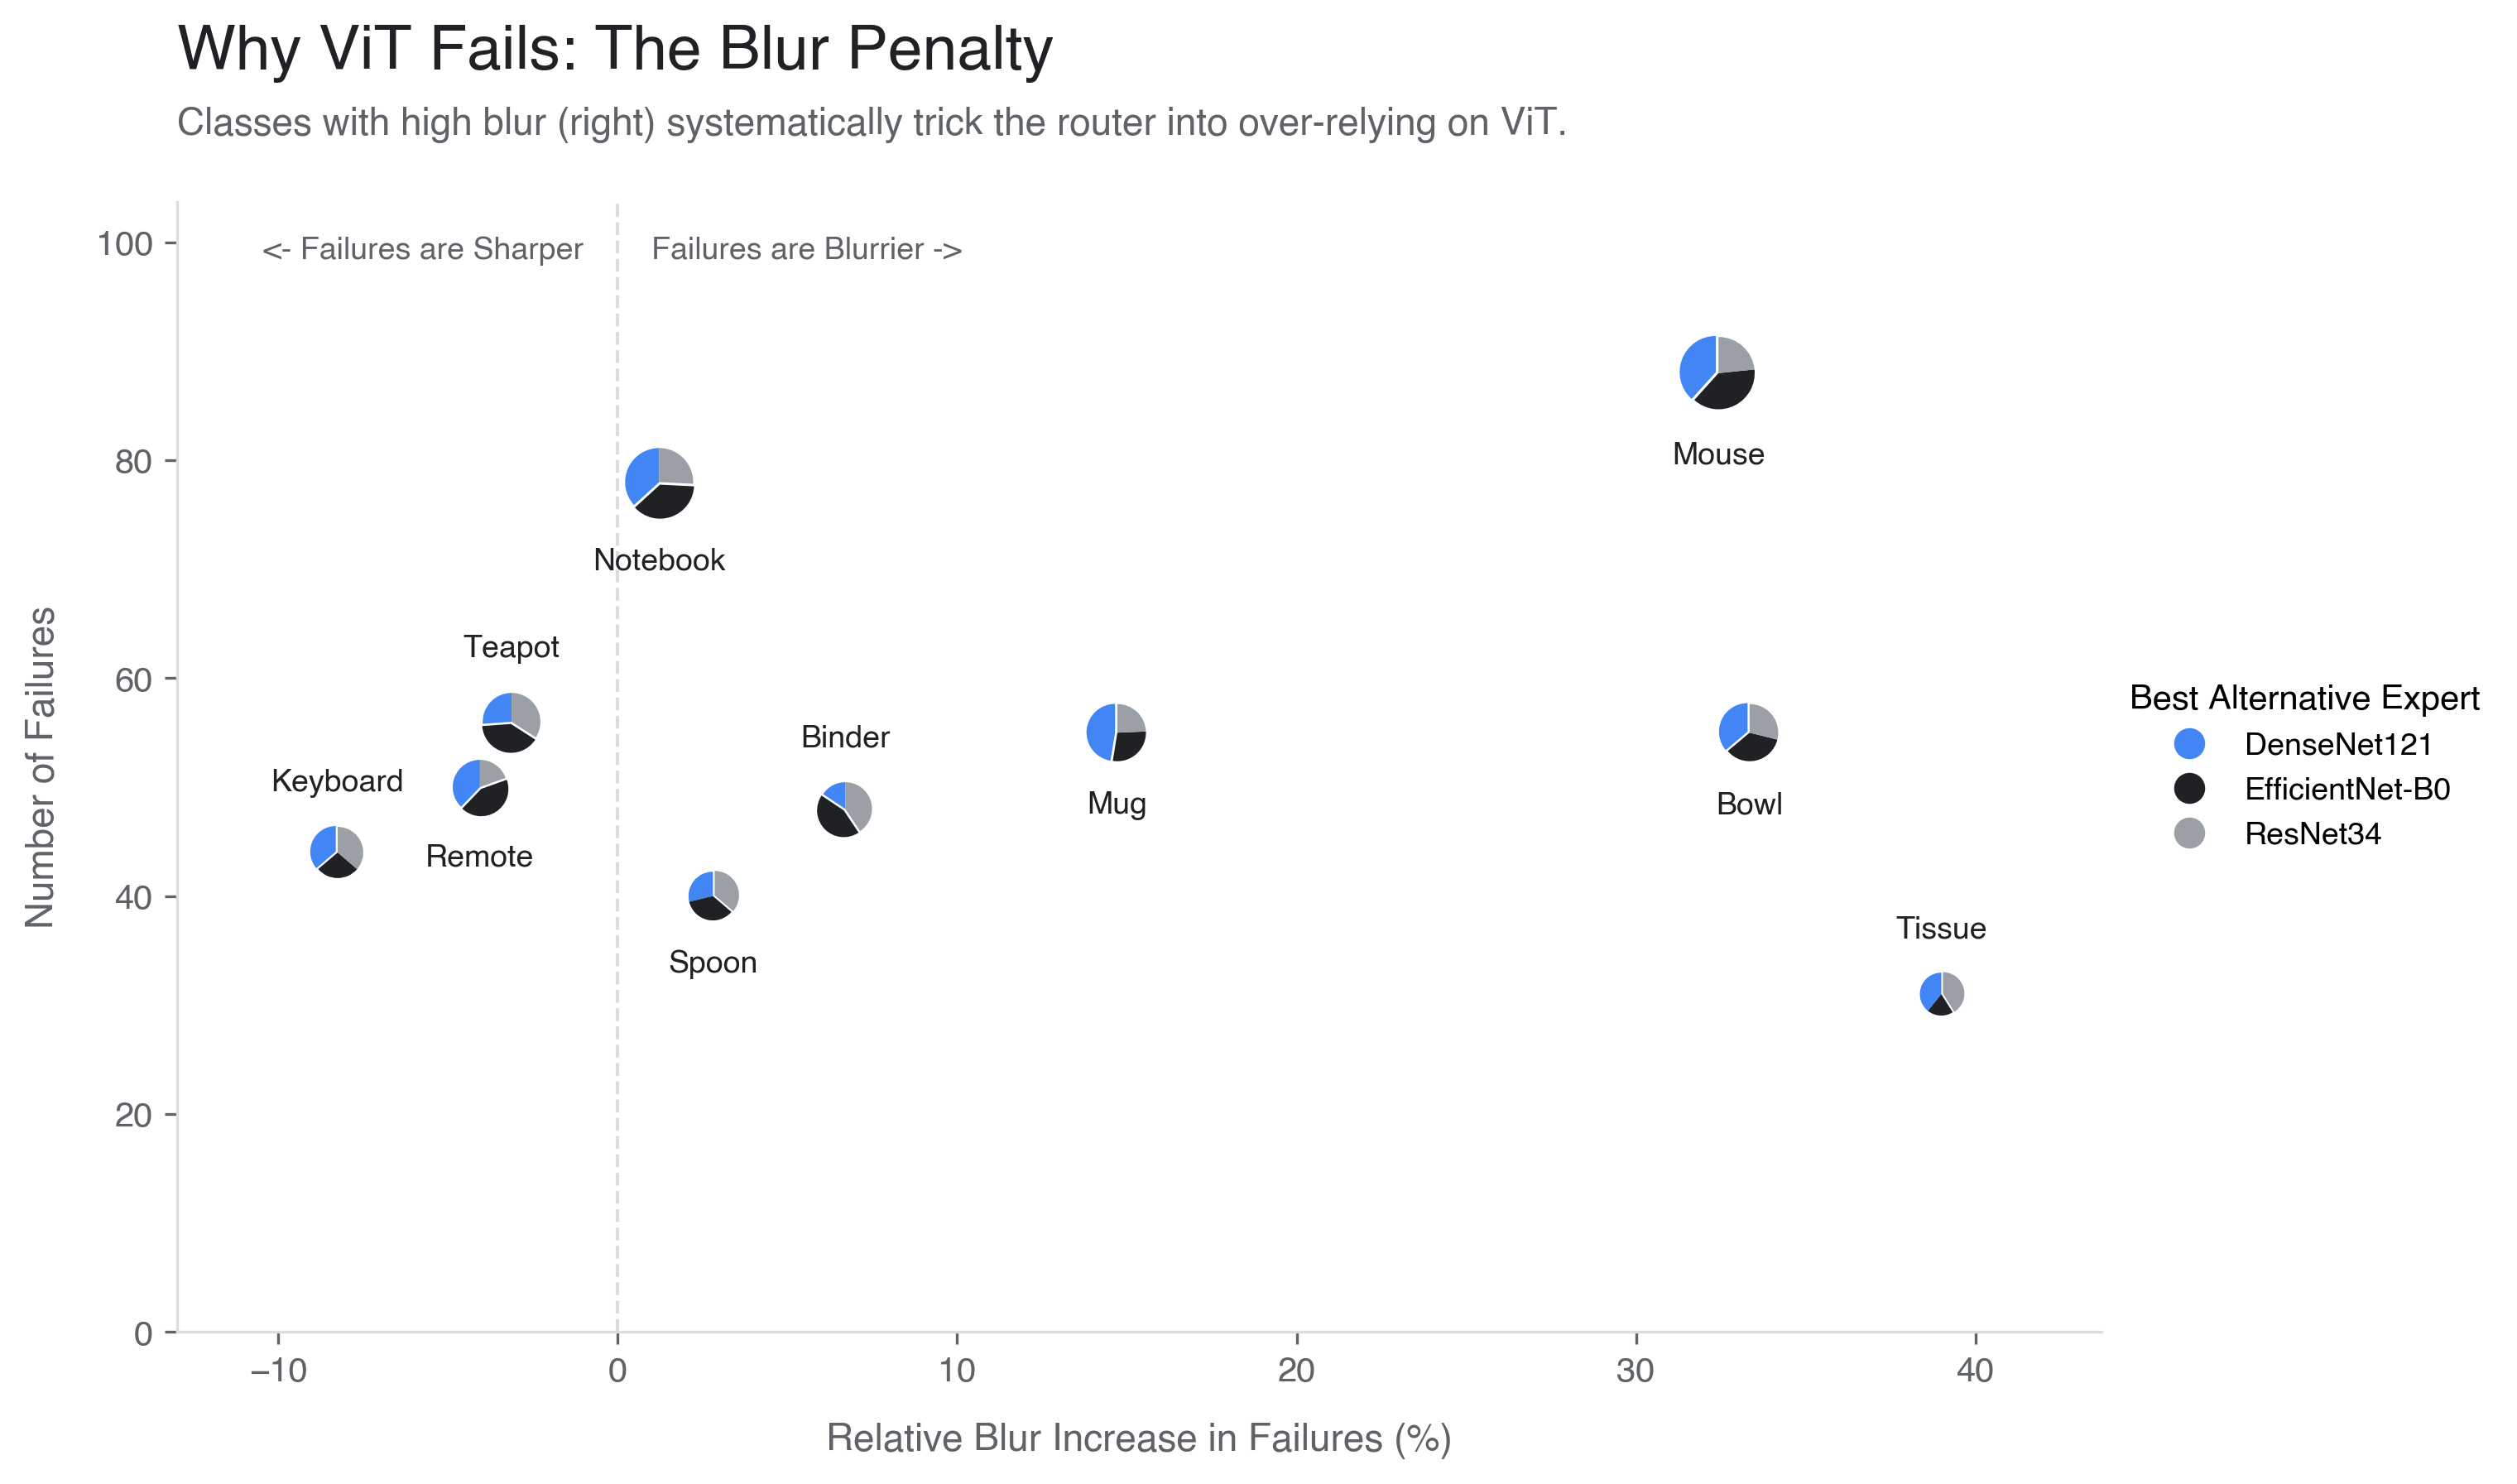
\includegraphics[width=1\linewidth]{xAI-StudentReportTemplate/figures/vit_failure_analysis_bubble.png}
    \rule[-.5cm]{0cm}{0cm}%
  }
  \caption{Analysis of ViT failure characteristics on the phone-captured dataset.
    The x-axis shows the relative increase in blur for failure cases compared to successful predictions, and the y-axis indicates the number of failures per class.
    Pie charts denote the alternative expert (DenseNet-121, EfficientNet-B0, or ResNet-34) that correctly predicts the label in these cases.}
  \label{fig:vit_bubble}
\end{figure}